%!TEX TS-program = xelatex
 
% Этот шаблон документа разработан в 2014 году
% Данилом Фёдоровых (danil@fedorovykh.ru) 
% для использования в курсе 
% <<Документы и презентации в \LaTeX>>, записанном НИУ ВШЭ
% для Coursera.org: http://coursera.org/course/latex .
% Исходная версия шаблона --- 
% https://www.writelatex.com/coursera/latex/5.2.2
 
\documentclass[a4paper,12pt]{article}
 
%%% Работа с русским языком
\usepackage[english,russian]{babel}   %% загружает пакет многоязыковой вёрстки
\usepackage{fontspec}      %% подготавливает загрузку шрифтов Open Type, True Type и др.
\defaultfontfeatures{Ligatures={TeX},Renderer=Basic}  %% свойства шрифтов по умолчанию
\setmainfont[Ligatures={TeX,Historic}]{Times New Roman} %% задаёт основной шрифт документа
\setsansfont{Comic Sans MS}                    %% задаёт шрифт без засечек
\setmonofont{Courier New}
\usepackage{indentfirst}
\frenchspacing
 
\renewcommand{\epsilon}{\ensuremath{\varepsilon}}
\renewcommand{\phi}{\ensuremath{\varphi}}
\renewcommand{\kappa}{\ensuremath{\varkappa}}
\renewcommand{\le}{\ensuremath{\leqslant}}
\renewcommand{\leq}{\ensuremath{\leqslant}}
\renewcommand{\ge}{\ensuremath{\geqslant}}
\renewcommand{\geq}{\ensuremath{\geqslant}}
\renewcommand{\emptyset}{\varnothing}
 
%%% Дополнительная работа с математикой
\usepackage{amsmath,amsfonts,amssymb,amsthm,mathtools} % AMS
\usepackage{icomma} % "Умная" запятая: $0,2$ --- число, $0, 2$ --- перечисление
 
%% Номера формул
%\mathtoolsset{showonlyrefs=true} % Показывать номера только у тех формул, на которые есть \eqref{} в тексте.
%\usepackage{leqno} % Нумерация формул слева
 
%% Свои команды
\DeclareMathOperator{\sgn}{\mathop{sgn}}
 
%% Перенос знаков в формулах (по Львовскому)
\newcommand*{\hm}[1]{#1\nobreak\discretionary{}
{\hbox{$\mathsurround=0pt #1$}}{}}
 
%%% Работа с картинками
\usepackage{graphicx}  % Для вставки рисунков
\graphicspath{{images/}{images2/}}  % папки с картинками
\setlength\fboxsep{3pt} % Отступ рамки \fbox{} от рисунка
\setlength\fboxrule{1pt} % Толщина линий рамки \fbox{}
\usepackage{wrapfig} % Обтекание рисунков текстом
 
%%% Работа с таблицами
\usepackage{array,tabularx,tabulary,booktabs} % Дополнительная работа с таблицами
\usepackage{longtable}  % Длинные таблицы
\usepackage{multirow} % Слияние строк в таблице
 
%%% Теоремы
\theoremstyle{plain} % Это стиль по умолчанию, его можно не переопределять.
\newtheorem{theorem}{Теорема}[section]
\newtheorem{proposition}[theorem]{Утверждение}
 
\theoremstyle{definition} % "Определение"
\newtheorem{corollary}{Следствие}[theorem]
\newtheorem{problem}{Задача}[section]
 
\theoremstyle{remark} % "Примечание"
\newtheorem*{nonum}{Решение}
 
%%% Программирование
\usepackage{etoolbox} % логические операторы
 
 
%%% Страница
\usepackage{extsizes} % Возможность сделать 14-й шрифт
\usepackage{geometry} % Простой способ задавать поля
	\geometry{top=5mm}
	\geometry{bottom=15mm}
	\geometry{left=5mm}
	\geometry{right=5mm}
 %
%\usepackage{fancyhdr} % Колонтитулы
% 	\pagestyle{fancy}
 	%\renewcommand{\headrulewidth}{0pt}  % Толщина линейки, отчеркивающей верхний колонтитул
% 	\lfoot{Нижний левый}
% 	\rfoot{Нижний правый}
% 	\rhead{Верхний правый}
% 	\chead{Верхний в центре}
% 	\lhead{Верхний левый}
%	\cfoot{Нижний в центре} % По умолчанию здесь номер страницы
 
\usepackage{setspace} % Интерлиньяж
%\onehalfspacing % Интерлиньяж 1.5
%\doublespacing % Интерлиньяж 2
%\singlespacing % Интерлиньяж 1
 
\usepackage{lastpage} % Узнать, сколько всего страниц в документе.
 
\usepackage{soul} % Модификаторы начертания
 
\usepackage{hyperref}
\usepackage[usenames,dvipsnames,svgnames,table,rgb]{xcolor}
\hypersetup{				% Гиперссылки
    unicode=true,           % русские буквы в раздела PDF
    pdftitle={Заголовок},   % Заголовок
    pdfauthor={Автор},      % Автор
    pdfsubject={Тема},      % Тема
    pdfcreator={Создатель}, % Создатель
    pdfproducer={Производитель}, % Производитель
    pdfkeywords={keyword1} {key2} {key3}, % Ключевые слова
    colorlinks=true,       	% false: ссылки в рамках; true: цветные ссылки
    linkcolor=red,          % внутренние ссылки
    citecolor=black,        % на библиографию
    filecolor=magenta,      % на файлы
    urlcolor=cyan           % на URL
}
 
\usepackage{csquotes} % Еще инструменты для ссылок
 
%\usepackage[style=authoryear,maxcitenames=2,backend=biber,sorting=nty]{biblatex}
 
\usepackage{multicol} % Несколько колонок
 
\usepackage{tikz} % Работа с графикой
\usepackage{pgfplots}
\usepackage{pgfplotstable}
 
\author{Батарин Егор}
\title{Поляризация}
\date{\today}
 
\begin{document} % конец преамбулы, начало документа
 
\maketitle
 
\begin{abstract}
   Цель работы: ознакомление с методами получения и анализа поляризованного света.
\end{abstract}
 
\section{Теория}
\begin{enumerate}
\item Понятие эллиптической, круговой и линейной поляризации.

Покажем, что монохроматическая электромагнитная волна, распространяющуяся в вакууме, является поляризованной. Пусть она распространяется по оси $z$. Имеем
\[ \operatorname{div}\vec{E} =  \frac{\partial E_x}{\partial x} +  \frac{\partial E_y}{\partial y} +  \frac{\partial E_z}{\partial z}\ = 0 \]
C учетом этого и $ \frac{\partial E_x}{\partial x} = \frac{\partial E_y}{\partial y} = 0 \Rightarrow  \frac{\partial E_z}{\partial z}\ = 0$. Далее, из уравнения циркуляции магнитного поля имеем
\[  \left(\operatorname{rot}\vec{H}\right)_z =  \frac{\partial H_y}{\partial y} +  \frac{\partial H_x}{\partial x}  = \frac{1}{c}\frac{\partial E_z}{\partial t} \]
Поэтому $\frac{\partial E_z}{\partial t} = 0$ и $E_z = \operatorname{const} = 0$ - без ограничения общности. Учитывая, что $E_z = H_z = 0$, запишем уравнения для $\vec{E}$ и $\vec{H}$. Получатся две независимые системы уравнений:

\begin{equation*}
\begin{cases}
\left(\operatorname{rot}\vec{E}\right)_y = \frac{\partial E_x}{\partial z}\ = -\frac{1}{c}\frac{\partial H_y}{\partial t}
\\
\left(\operatorname{rot}\vec{E}\right)_x = \frac{\partial E_y}{\partial z}\ = \frac{1}{c}\frac{\partial H_x}{\partial t}
\end{cases}
\begin{cases}
\left(\operatorname{rot}\vec{H}\right)_x = -\frac{\partial H_y}{\partial z}\ = \frac{1}{c}\frac{\partial E_x}{\partial t}
\\
\left(\operatorname{rot}\vec{H}\right)_y = \frac{\partial H_x}{\partial z}\ = \frac{1}{c}\frac{\partial E_y}{\partial t}
\end{cases}
\end{equation*} 
Из этой системы получается 
\begin{equation*}
\begin{cases}
E_x = \mp H_y = f_x(ct \pm z)
\\
E_y = \pm H_x = f_y(ct \pm z)
\end{cases}
\end{equation*}
Здесь $f_x$ и $f_y$ - произвольные функции. В частности, для монохроматических волн получаем уравнение плоско-поляризованной волны:
\begin{equation*}
\begin{cases}
E_x = H_y = A_x\cos(\omega t -kz+\phi_x)
\\
E_y = - H_x = A_y\cos(\omega t -kz + \phi_y )
\end{cases}
\end{equation*}

В общем случае вектор $\left(E_x,E_y\right)$ вращается по эллипсу - эллиптическая поляризация. Если эллипс является окружностью, то мы имеем дело с круговой поляризацией, если вырождается в отрехок - линейной поляризацией.

\item Получение эллиптически поляризованного света

Пусть есть источник линейно-поляризованного света. С помощью двояко-преломляющей пластины, из него можно получить эллиптически поляризованный свет. Для этого нужно пустить исходные волны по двух взаимо-перпенликулярным главным направлениям пластинки (главные волны), они будут распространяться с разными скоростями и на выходе получится сдвиг фаз. Рассмотрим частные случаи сдвига фаз $\Delta\phi$:

1) $\Delta\phi = 2\pi$, пластинка в длину волны $\lambda$. Получается линейно-поляризованная волна на выходе.

2) $\Delta\phi = \pi$, пластинка в длину волны $\lambda/2$. На выходе снова получается линейно-поляризованная волна, но теперь направление колебаний выходного линейно-поляризованного света является зеркальным отражением направления колебаний входного линейно-поляризованного света относительно одного из главных направлений пластинки.

3)  $\Delta\phi = \pi/2$, пластинка в длину волны $\lambda/4$. Получается эллиптически поляризованный свет, причем его главные оси совпадают с главными направлениями кристаллической решетки.
\end{enumerate}
\section{Выполнение}
\begin{enumerate}
   \item Определение разрешенных направлений поляроидов.
   
   	Минимальная интенсивность света в установке с черным зеркалом достигается при угле поляроида $310^{\circ} \pm 10^{\circ}$ - выставлена горизонтальная поляризация.
   	
   	 \begin{figure}[h!]
   		\center{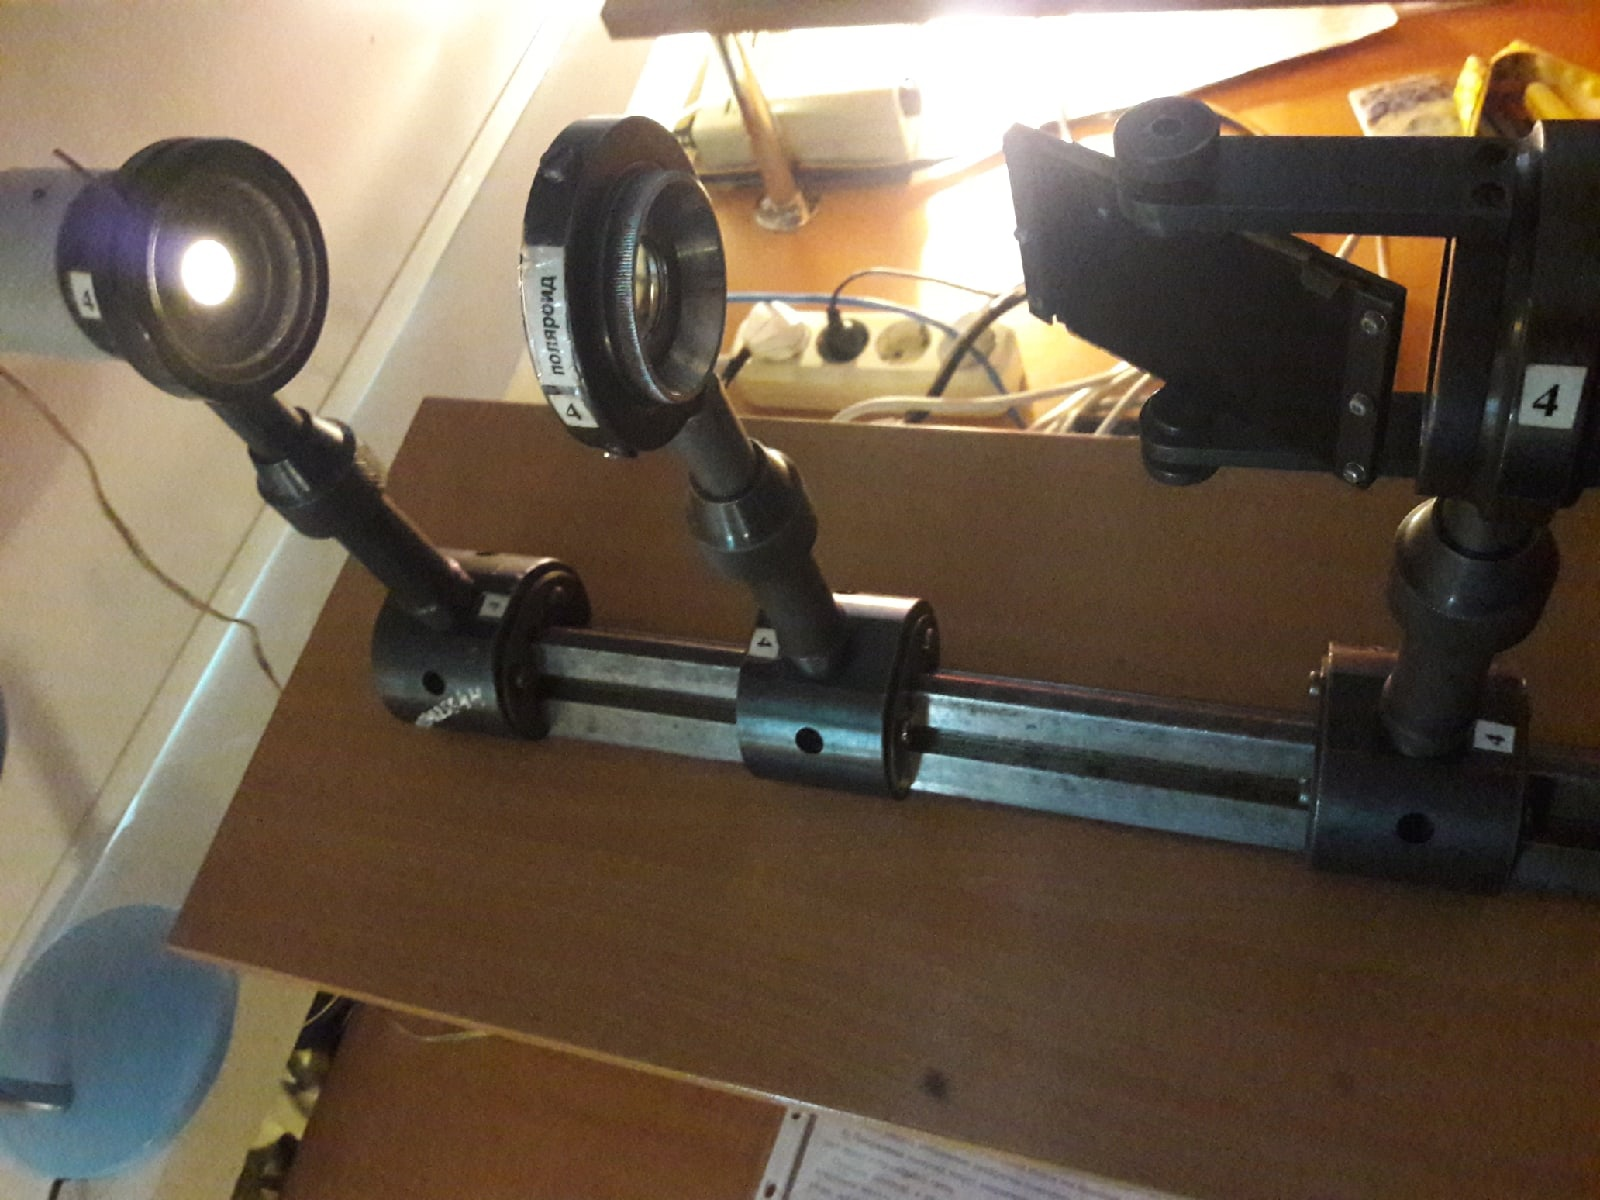
\includegraphics[scale = 0.1]{1.jpg}}
   		\caption{Положение зеркала под углом Брюстера. Настройка горизонтальной поляризации.}
   	\end{figure}
   
   
   Если заменить зеркало на второй поляроид и поставить на $220^{\circ} \pm 10^{\circ}$, то интенсивность света, прошедшего через скрещенные поляроиды, будет минимальна.
	
	\begin{figure}[h!]
		\center{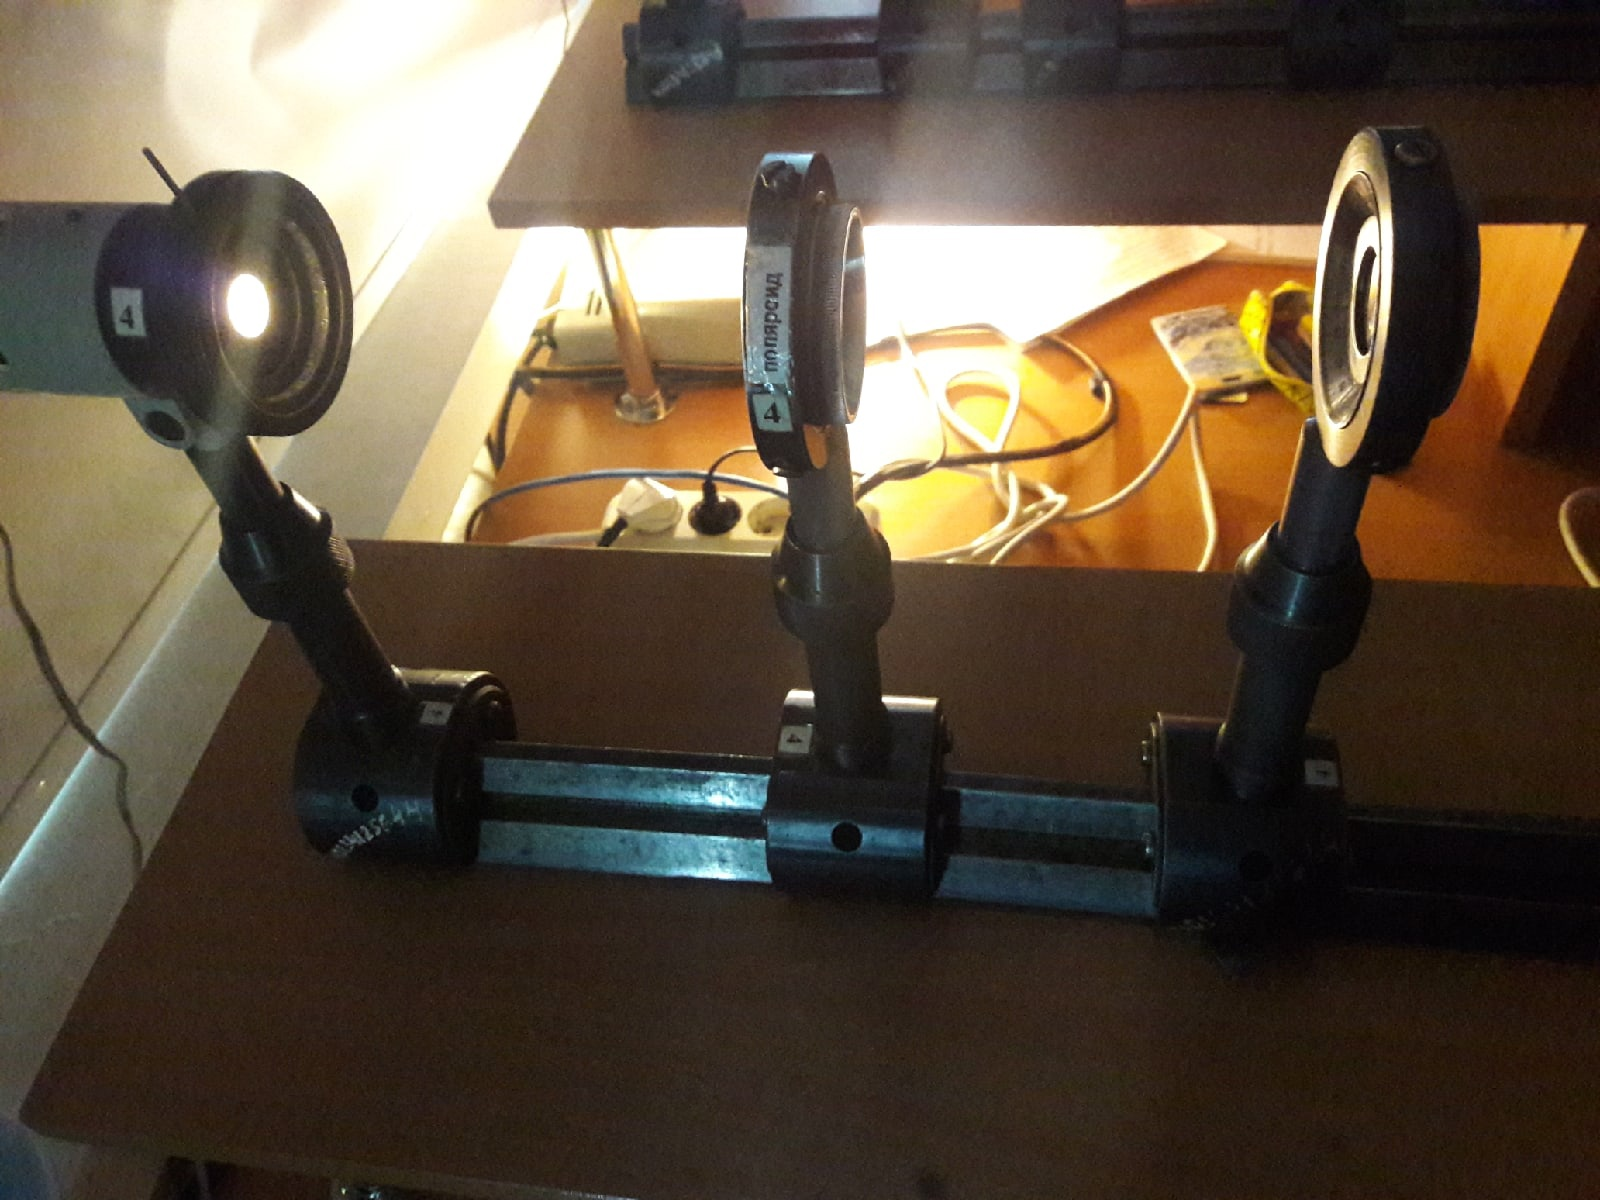
\includegraphics[scale = 0.1]{2.jpg}}
		\caption{Настройка второго поляроида.}
	\end{figure}
	
	\item Определение показателя преломления (угла Брюстера) для эбонита.
	 
	 Выбираем начало отсчета по лимбу - $195^{\circ} \pm 5^{\circ}$. Риска на минимальной интенсивности - $250^{\circ} \pm 5^{\circ}$. Тогда для естественного света получаем показатель преломления $n_1 = \tg(55^{\circ}) \approx 1.42 \pm \left.\frac{\partial \tg(\phi)}{\partial \phi}\right|_{\phi = 55^{\circ}}\Delta\phi=0.28 $. Если поставить зеленый фильтр, то получится угол $248^{\circ} \pm 5^{\circ}$ и соответвующий ему показатель преломления $n_2 = \tg(53^{\circ}) \approx 1.32 \pm 0.24$.
	 \begin{figure}[h!]
	 	\center{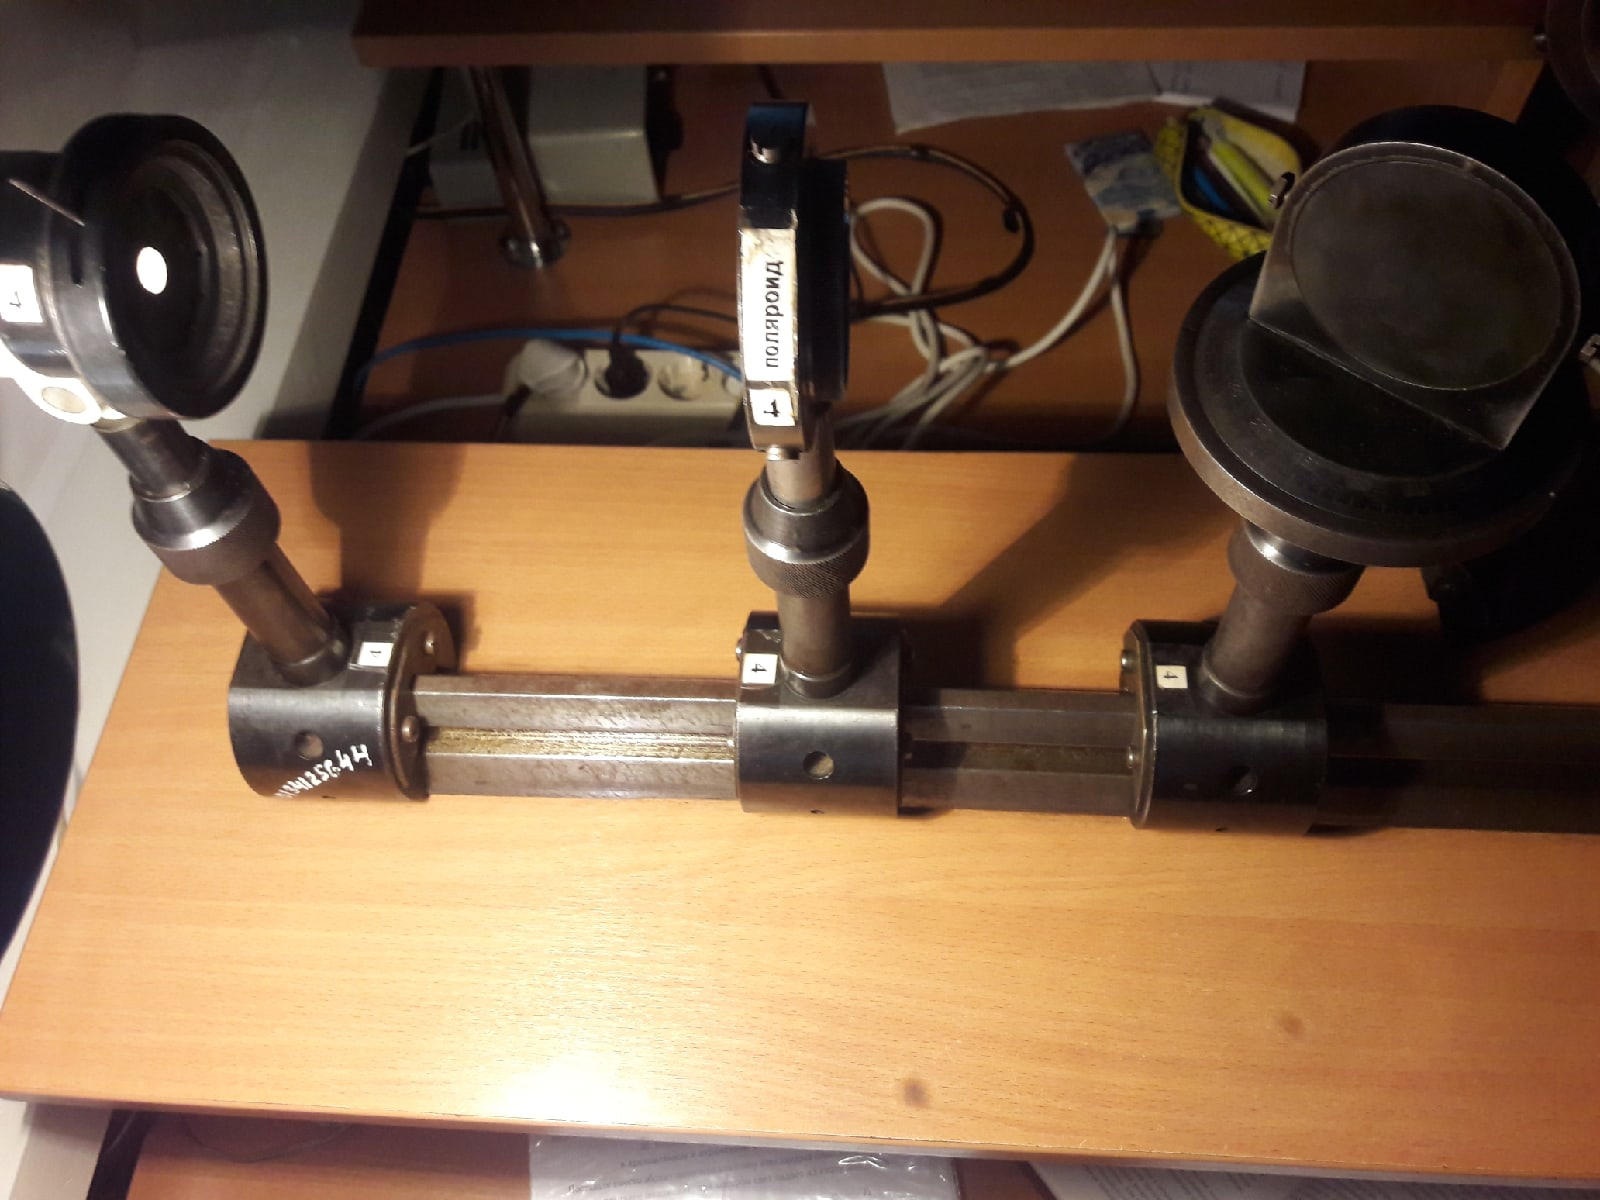
\includegraphics[scale = 0.1]{3.jpg}}
	 	\caption{Опыты с эбонитом.}
	 \end{figure}
	 
	\item Исследование поляризации света в преломленном и отраженном от стопы лучах.
	
	Устанавливаем стопу на минимальную интенсивность под углом Брюстера. Если на пути отраженного света поставить поляроид с горизонтальным разрешенным направлением, то интенсивность света сильно уменьшится. Если на пути отраженного света поставить поляроид с вертикальным разрешенным направлением, то интенсивность света не изменится. Следовательно, вектор $\vec{E}$ отраженного света направлен вертикально. В случае преломленного света получается обратный результат. Следовательно, вектор $\vec{E}$ преломленного света направлен горизонтально.
	
	\item Определение главных направлений двоякопреломляющих пластин.
	
	Главное направление пластинки совпадает с разрешенными направлениями поляризоидов только тогда, когда интенсивность света, проходящего через систему, максимальна. 
	Для пластинки с кружочком получается углы $160, 70, 340, 250 \pm 5$ градусов - повторяется каждые $90$ градусов. Для пластинки без кружочка получаются те же углы.
	
	\item Выделение пластин $\lambda/2$ и $\lambda/4$.

	Добавляем зеленый фильтр.
	
	Эллиптическая поляризация - в этом случае если крутить второй поляризатор, то интенсивность света не будет меняться слишком сильно. Это происходит для пластины с кружочком. Значит это пластина в $\lambda/4$.
	
	\begin{figure}[h!]
		\center{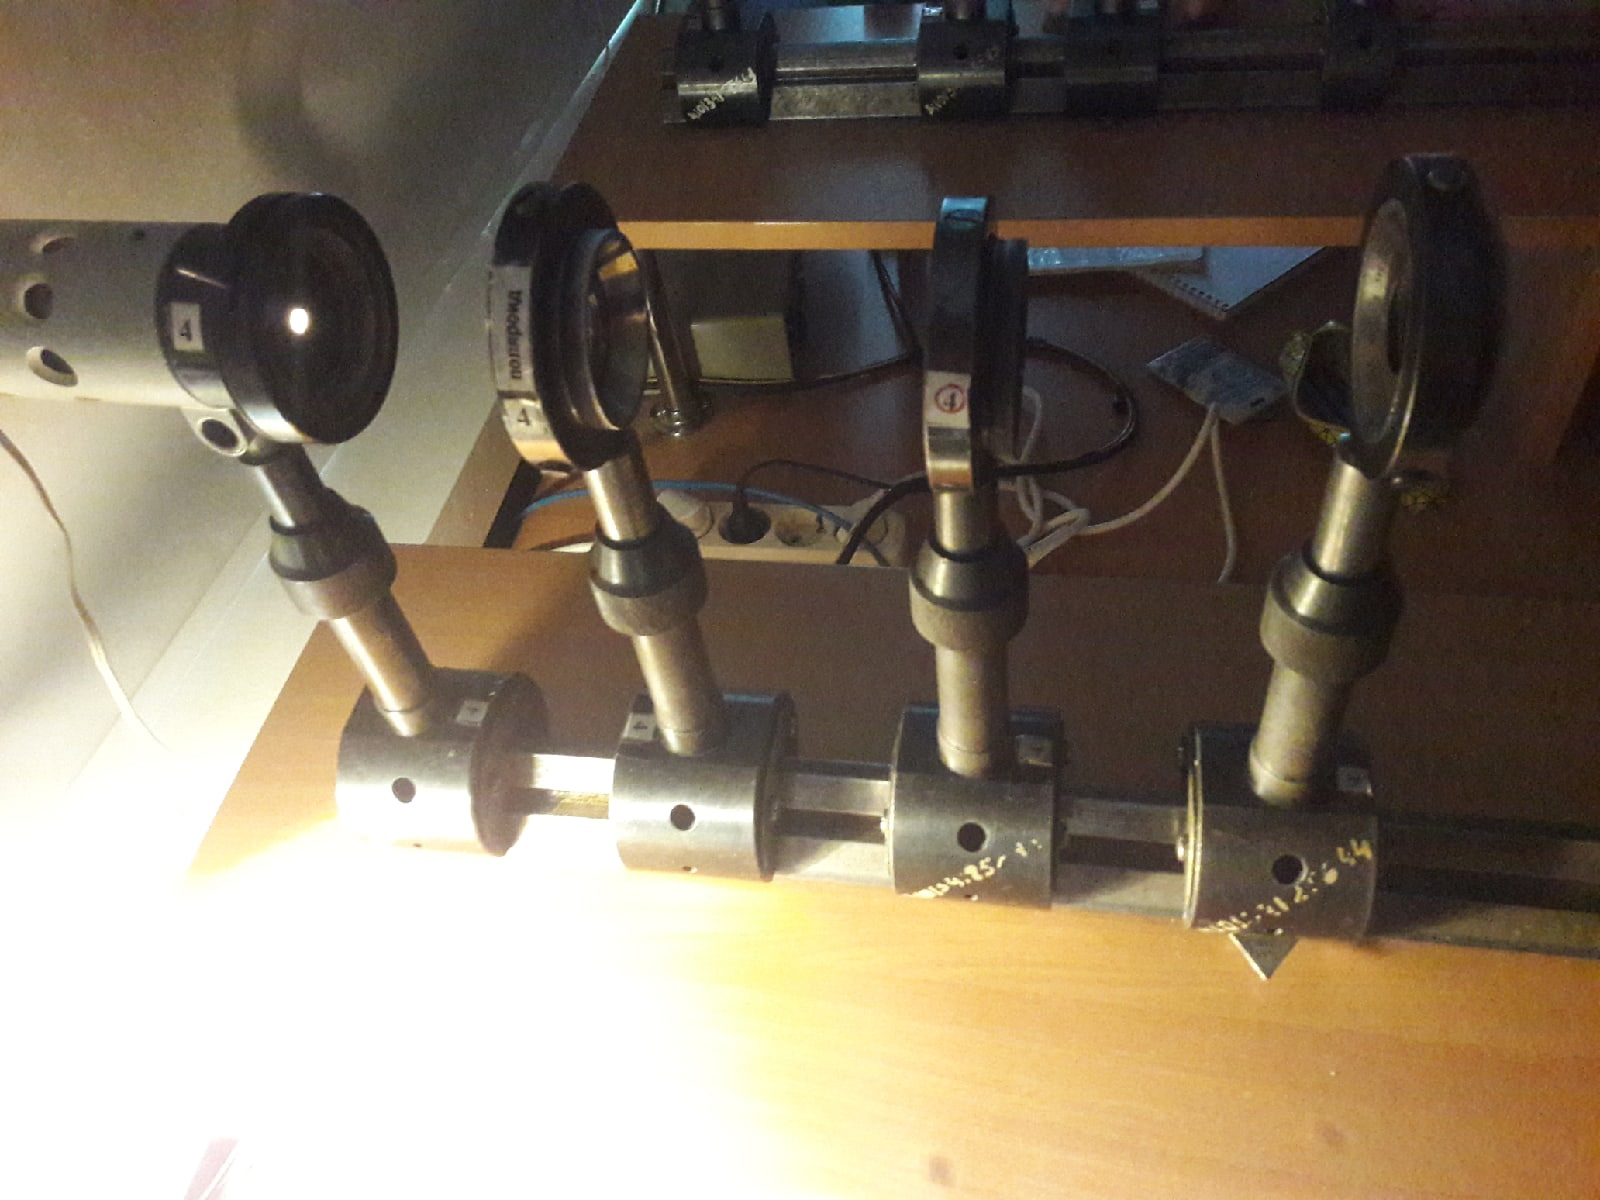
\includegraphics[scale = 0.1]{4.jpg}}
		\caption{Определение толщины пластины по поляризационному характеру выходного света.}
	\end{figure}
	
	Если интенсивность меняется значительно и можно отчетливо наблюдать минимумы и максимумы, то мы имеем дело с линейной поляризацией. Такое происходит с пластиной без кружочка. Значит это пластина в $\lambda/2$.

	\item Определение быстрой и медленной оси в пластинке $\lambda/4$.
	
	Цвет заказался зеленовато-голубым, когда у пластинки $\lambda/4$ и $\lambda$ совпадали главные направления, соответсвующие большей скорости распространения. Это происходит потому, что при освещении белым светом этих пластинок погасилась зеленая часть спектра, а красная - гасится.
	
	\begin{figure}[h!]
		\center{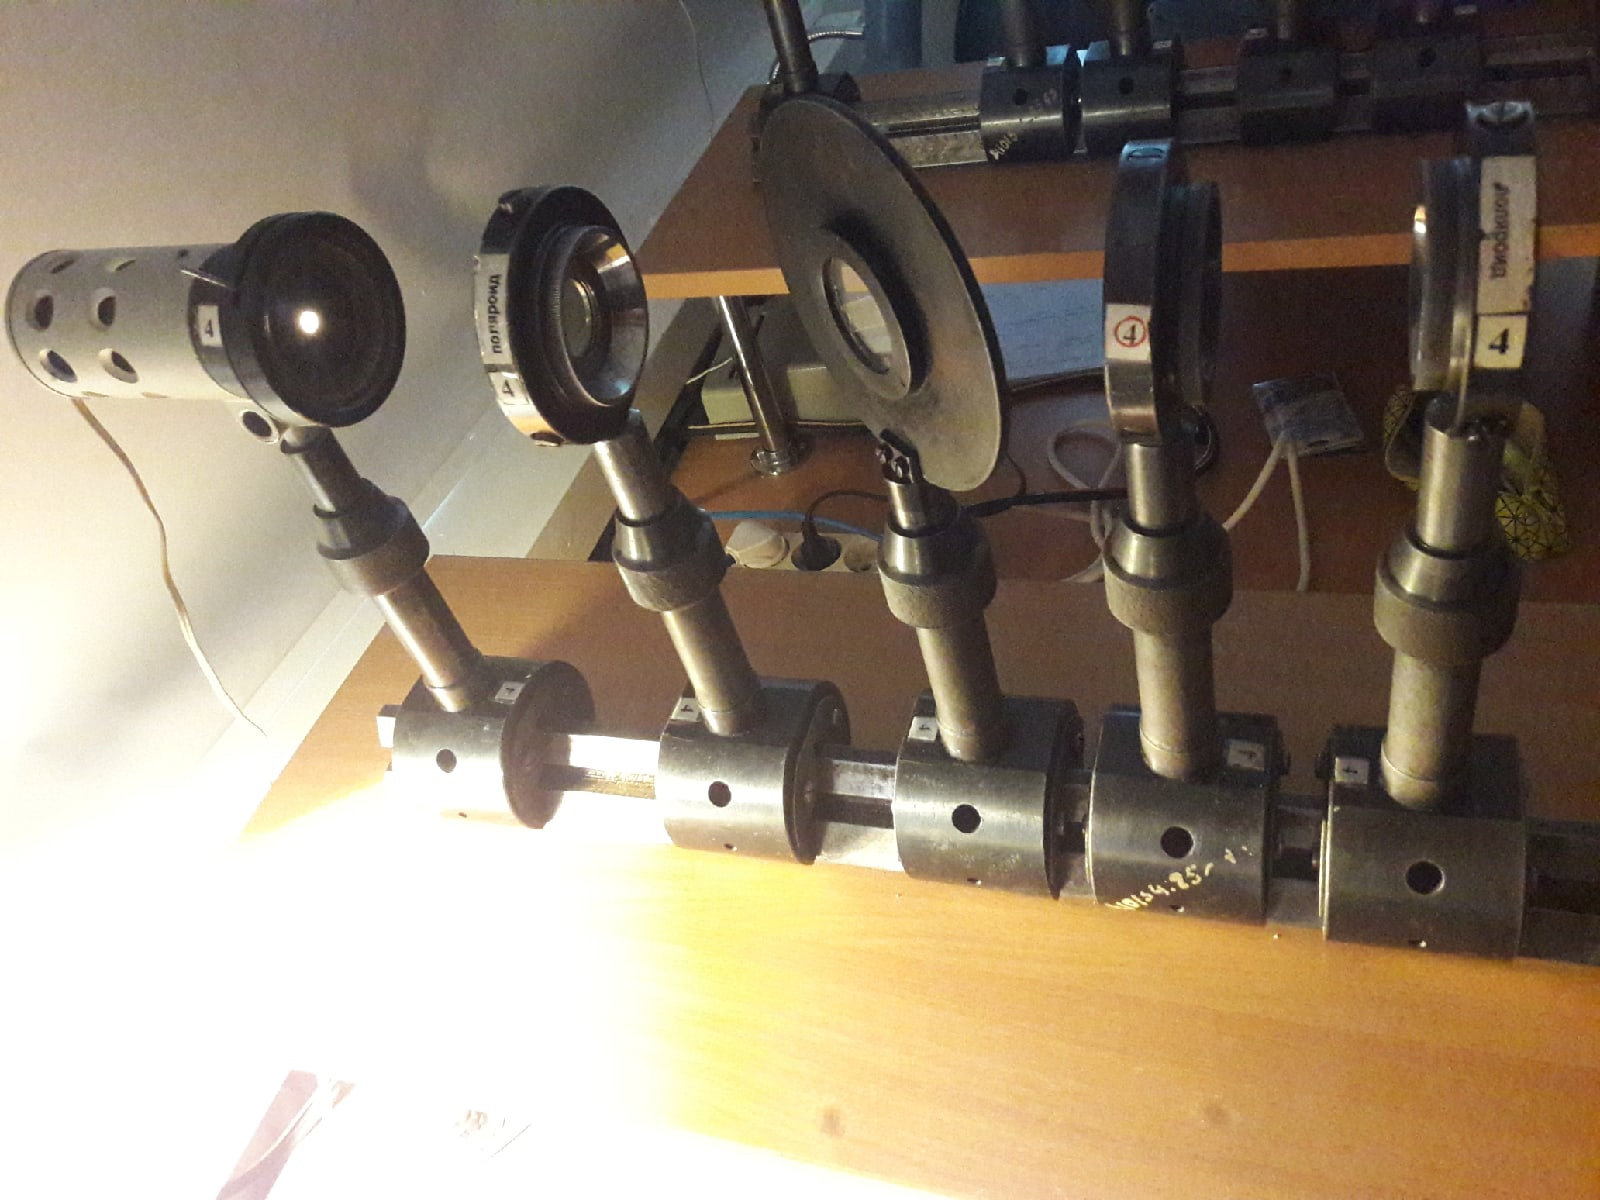
\includegraphics[scale = 0.1]{5.jpg}}
		\caption{Опыты с $\lambda$ пластинкой.}
	\end{figure}
	
	
	Цвет приобрел оранжеов-желтую окруаску, когда эти главные направления оказывались перпендикулярными. В этом случае гасится фиолетово-голубая часть спектра.
	
	\item Интерференция поляризованных лучей.
	
	Зафиксируем два скрещенных поляризоида. Если вращать мозаичную сляюдяную пластинку, то в 4 квадратиках наблюдается красный цвет, в 2 - зеленый, в оставшихся 2 - желтый. При этом яркость этих цветов синхронно меняется от минимального значения до максимального.
	
	\begin{figure}[h!]
		\center{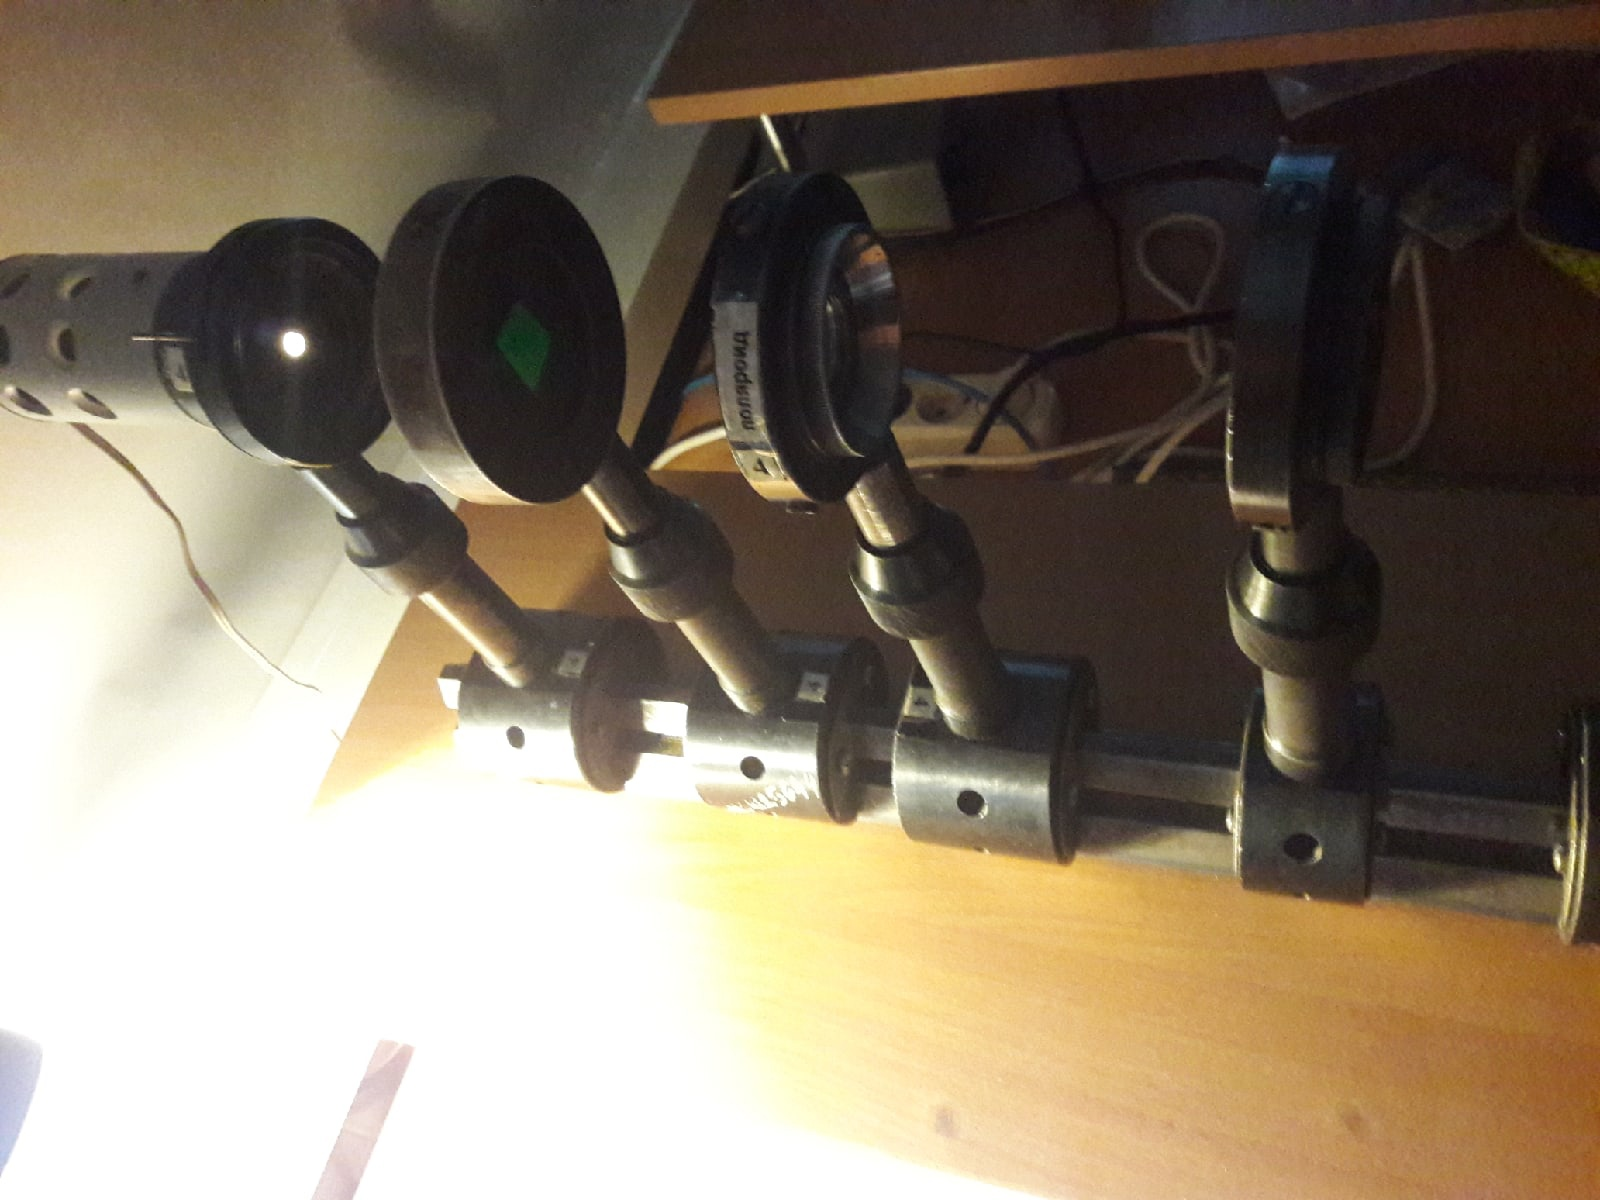
\includegraphics[scale = 0.1]{6.jpg}}
		\caption{Эксперименты с мозаичной пластинкой.}
	\end{figure}

	Если вращать второй поляризоид, то яркость меняться не будет, но будут меняться цвета в квадратиках. В определенный момент времени в квадратах наблюдается естественный свет, без выделенных цветов.
	
	
\end{enumerate}
\end{document} % конец документа
 